\subsubsection{Initial Value (updated to assemble right to left like the other gadgets)}
We begin by encoding $\counterstart$ with the Seed unit. It has $\ceil*{\frac{d}{3}}$ digit regions.
Each digit region has three digits, except for the most significant digit region (MSR) which has $d \mod 3$
if $d \mod 3 \not= 0$, otherwise it has 3 digits.

\begin{figure}[H]
    \centering
    \begin{subfigure}[t]{0.24\textwidth}
        \centering
        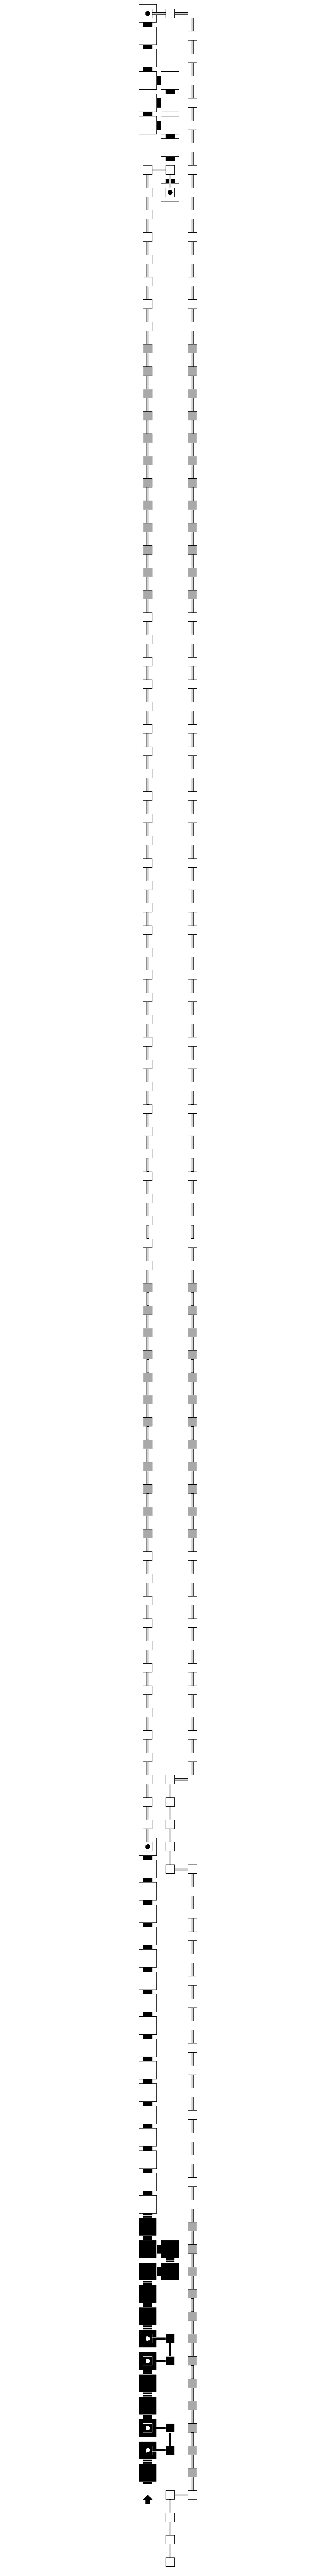
\includegraphics[width=0.24\textwidth]{initial_value_case1_msr}
        \caption{\label{fig:initial_case2} MSR case 1}
    \end{subfigure}%
    ~
    \begin{subfigure}[t]{0.24\textwidth}
        \centering
        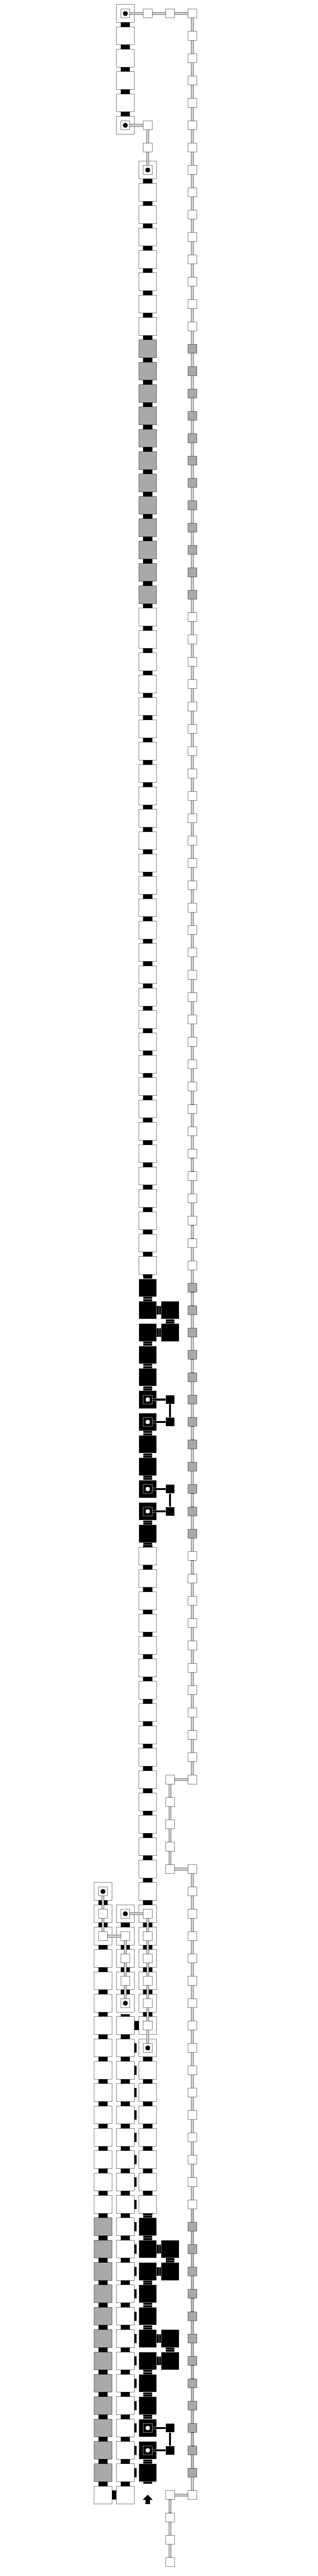
\includegraphics[width=0.24\textwidth]{initial_value_case2_msr}
        \caption{\label{fig:initial_case2} MSR case 2}
    \end{subfigure}%
    ~
    \begin{subfigure}[t]{0.24\textwidth}
        \centering
        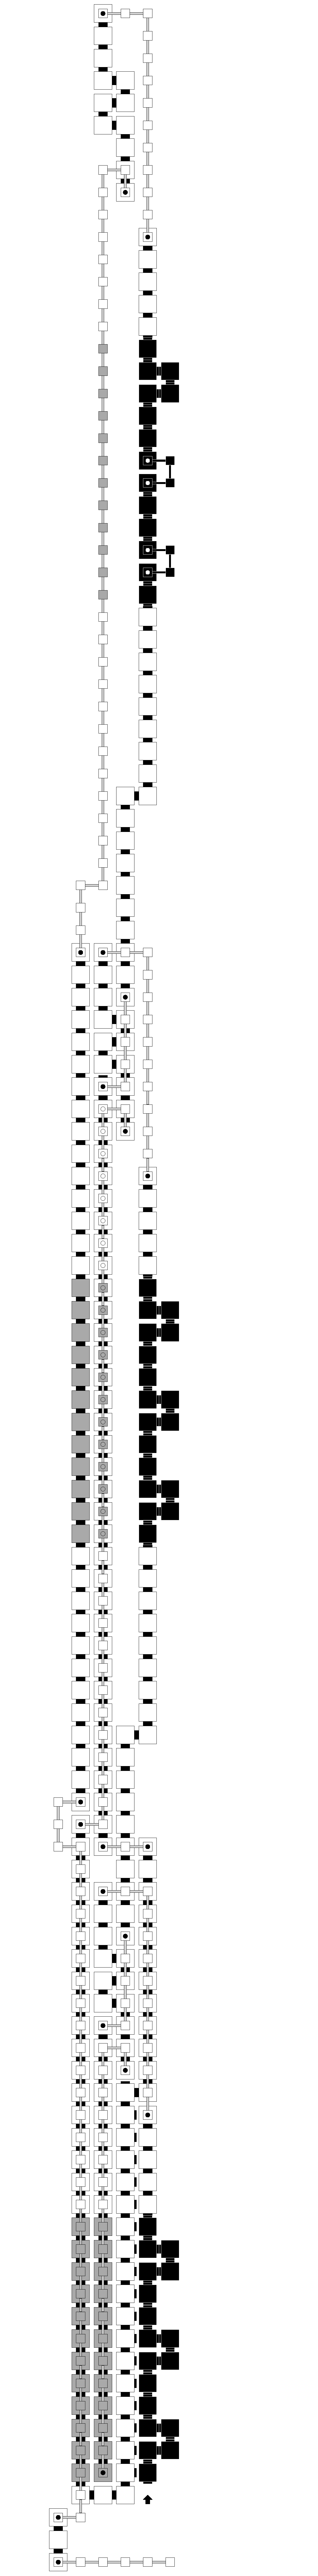
\includegraphics[width=0.24\textwidth]{initial_value_case3_msr}
        \caption{\label{fig:initial_case3} MSR case 3}
    \end{subfigure}%
    ~
    \begin{subfigure}[t]{0.24\textwidth}
        \centering
        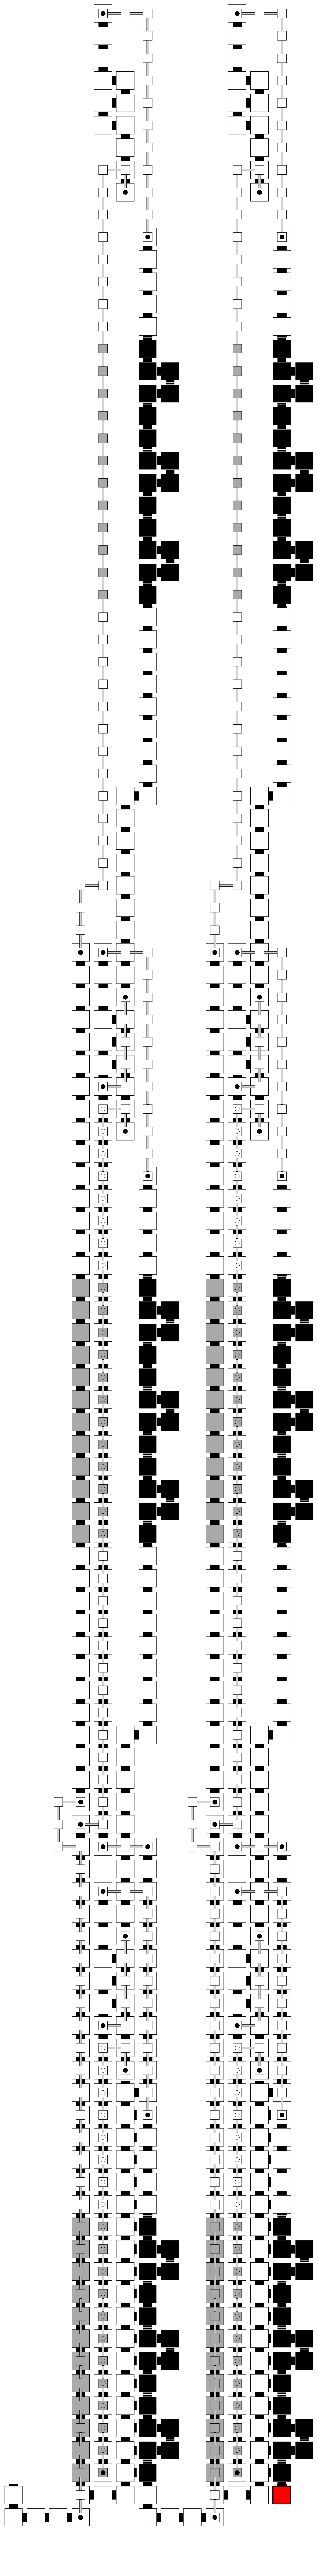
\includegraphics[width=0.24\textwidth]{initial_value_general}
        \caption{\label{fig:initial_general} Two general regions. Seed tile is the red tile in the bottom right}
    \end{subfigure}%
    \caption{\label{fig:initial_value_assemblies} Overviews of the initial assemble}
\end{figure}


Let $i = 0$, be the index of a digit in $\counterstart$,
\begin{itemize}
    \item Create
    $\begin{aligned}[t]
        {\tt Seed}(&\left\langle {\tt Write}, 1, {\tt seed}, 0, 0 \right\rangle \; )
    \end{aligned}$
\end{itemize}


General non-MSR digit region shown in Figure~\ref{fig:initial_general}.

While $i$ is not a digit in the MSR:

\begin{itemize}
    \item {\tt Start}:

    \item {\tt Digit}: for each $j=0,\ldots,l-1$ and each $b$ in $bin(C_0[i])[j]$:
    \begin{itemize}
        \item if $j = 0$: create
        $\begin{aligned}[t]
            \dwriter(&\left\langle {\tt Write}, 1, {\tt seed}, i, j \right\rangle, \left\langle {\tt Write}, 1, {\tt seed}, i, j + 1 \right\rangle \;)
        \end{aligned}$\\from the general gadget shown in Figure~\ref{fig:write_0}.

        \item if $j = 1$: create
        $\begin{aligned}[t]
            \dwriter(&\left\langle {\tt Write}, 1, {\tt seed}, i, j \right\rangle, \left\langle {\tt Write}, 1, {\tt seed}, i, j + 1 \right\rangle \;)
        \end{aligned}$\\from the general gadget shown in Figure~\ref{fig:write_0}.

        \item if $1 < j < l-1$: create
        $\begin{aligned}[t]
            \dwriter(&\left\langle {\tt Write}, 1, {\tt seed}, i, j \right\rangle, \left\langle {\tt Write}, 1, {\tt seed}, i, j + 1 \right\rangle \;)
        \end{aligned}$\\from the general gadget shown in Figure~\ref{fig:write_0} if $b = 0$ or Figure~\ref{fig:write_1} if $b = 1$.

        \item if $j = l-1$: create
        $\begin{aligned}[t]
            \dwriter(&\left\langle {\tt Write}, 1, {\tt seed}, i, j \right\rangle, \left\langle {\tt DigitTop}, 1, {\tt seed}, i \right\rangle \;)
        \end{aligned}$\\from the general gadget shown in Figure~\ref{fig:write_0} if $b = 0$ or Figure~\ref{fig:write_1} if $b = 1$.
    \end{itemize}


    \item {\dtop}: the following statements create the gadget shown in Figure~\ref{fig:digit_top_general}.
    \begin{itemize}
        \item Create
        $\begin{aligned}[t]
            {\tt North\_Line5}(& \left \langle {\tt DigitTop},  1, {\tt seed}, i \right\rangle,
                                 \left \langle {\tt DigitTopA}, 1, {\tt seed}, i \right\rangle \;)
        \end{aligned}$\\ from the micro-gadget shown in Figure~\ref{fig:north_line}.

        \item Create
        $\begin{aligned}[t]
            {\tt Topper}(& \left\langle {\tt DigitTopA}, 1, {\tt seed}, i \right\rangle,
                           \left\langle {\tt DigitTopB}, 1, {\tt seed}, i \right\rangle \;)
        \end{aligned}$\\ from the micro-gadget shown in Figure~\ref{fig:topper_gen}.

        \item Create
        $\begin{aligned}[t]
            {\tt South\_Line4\textit{l}}(& \left\langle {\tt DigitTopB}, 1, {\tt seed}, i\right\rangle,
                                           \left\langle \returnpath,     1, {\tt seed}, i\right\rangle \;)
        \end{aligned}$\\ from the micro-gadget shown in Figure~\ref{fig:south_line}.
    \end{itemize}

    \item $i \gets i + 1$

    \item Create
    $\begin{aligned}[t]
            \returnfromdigit(&\left\langle \returnpath,      1, {\tt seed}, i - 1\right\rangle,
                              \left\langle {\tt SecondWarp}, 2, {\tt seed}, i    \right\rangle \;)
    \end{aligned}$\\ (single-tile)

    \item Create
    $\begin{aligned}[t]
        \secondwarp(&\left\langle {\tt SecondWarp}, 2, {\tt seed}, i \right\rangle,
                     \left\langle {\tt PostWarp},   2, {\tt seed}, i \right\rangle \;)
    \end{aligned}$

    \item Create
    $\begin{aligned}[t]
        \postwarp(&\left\langle {\tt PostWarp}, 2, {\tt seed}, i    \right\rangle,
                   \left\langle {\tt Write},    2, {\tt seed}, i, 0 \right\rangle \;)
    \end{aligned}$\\ from the general gadget show in Figure~\ref{fig:post_warp_general_digit2and3}.

    \item {\tt Digit}: for each $j=0,\ldots,l-1$ and each $b$ in $bin(C_0[i])[j]$:
    \begin{itemize}
        \item if $j = 0$: create
        $\begin{aligned}[t]
            \dwriter(&\left\langle {\tt Write}, 2, {\tt seed}, i, j \right\rangle, \left\langle {\tt Write}, 2, {\tt seed}, i, j + 1 \right\rangle \;)
        \end{aligned}$\\from the general gadget shown in Figure~\ref{fig:write_0}.

        \item if $j = 1$: create
        $\begin{aligned}[t]
            \dwriter(&\left\langle {\tt Write}, 2, {\tt seed}, i, j \right\rangle, \left\langle {\tt Write}, 2, {\tt seed}, i, j + 1 \right\rangle \;)
        \end{aligned}$\\from the general gadget shown in Figure~\ref{fig:write_0}.

        \item if $1 < j < l-1$: create
        $\begin{aligned}[t]
            \dwriter(&\left\langle {\tt Write}, 2, {\tt seed}, i, j \right\rangle, \left\langle {\tt Write}, 2, {\tt seed}, i, j + 1 \right\rangle \;)
        \end{aligned}$\\from the general gadget shown in Figure~\ref{fig:write_0} if $b = 0$ or Figure~\ref{fig:write_1} if $b = 1$.

        \item if $j = l-1$: create
        $\begin{aligned}[t]
            \dwriter(&\left\langle {\tt Write}, 2, {\tt seed}, i, j \right\rangle, \left\langle {\tt DigitTop}, 2, {\tt seed}, i \right\rangle \;)
        \end{aligned}$\\from the general gadget shown in Figure~\ref{fig:write_0} if $b = 0$ or Figure~\ref{fig:write_1} if $b = 1$.
    \end{itemize}


    \item {\dtop}: the following statements create the gadget shown in Figure~\ref{fig:digit_top_general}.
    \begin{itemize}
        \item Create
        $\begin{aligned}[t]
            {\tt North\_Line5}(& \left \langle {\tt DigitTop},  2, {\tt seed} , i \right\rangle,
                                 \left \langle {\tt DigitTopA}, 2, {\tt seed} , i \right\rangle \;)
        \end{aligned}$\\ from the micro-gadget shown in Figure~\ref{fig:north_line}.

        \item Create
        $\begin{aligned}[t]
            {\tt Topper}(& \left \langle {\tt DigitTopA}, 2, {\tt seed}, i \right\rangle,
                           \left \langle {\tt DigitTopB}, 2, {\tt seed}, i \right\rangle \;)
        \end{aligned}$\\ from the micro-gadget shown in Figure~\ref{fig:topper_gen}.

        \item Create
        $\begin{aligned}[t]
            {\tt South\_Line4\textit{l}}(&\left\langle {\tt DigitTopB}, 2, {\tt seed}, i \right\rangle,
                                          \left\langle \returnpath,     2, {\tt seed}, i \right\rangle \;)
        \end{aligned}$\\ from the micro-gadget shown in Figure~\ref{fig:south_line}.
    \end{itemize}


    \item Create
    $\begin{aligned}[t]
        \returnfromdigit(&\left\langle \returnpath,    2, {\tt seed}, i \right\rangle,
                          \left\langle {\tt NextRead}, 2, {\tt seed}, i \right\rangle \;)
    \end{aligned}$\\ from the gadget in Figure~\ref{fig:return_from_digit2_oporseed}.


    \item $i \gets i + 1$

    \item Create
    $\begin{aligned}[t]
        \readnext(&\left\langle {\tt NextRead},  2, {\tt seed}, i - 1 \right\rangle,
                   \left\langle {\tt FirstWarp}, 3, {\tt seed}, i     \right\rangle \;)
    \end{aligned}$\\ from the general gadget shown in Figure~\ref{fig:read_next_2_seed}.

    \item Create
    $\begin{aligned}[t]
        \firstwarp(&\left\langle {\tt FirstWarp},  3, {\tt seed}, i \right\rangle,
                    \left\langle {\tt WarpBridge}, 3, {\tt seed}, i \right\rangle \;)
    \end{aligned}$

    \item Create
    $\begin{aligned}[t]
        \warpbridge(&\left\langle {\tt WarpBridge}, 3, {\tt seed}, i \right\rangle,
                     \left\langle {\tt SecondWarp}, 3, {\tt seed}, i \right\rangle \;)
    \end{aligned}$\\ from the general gadget shown in Figure~\ref{fig:warp_bridge_general}.

    \item Create
    $\begin{aligned}[t]
        \secondwarp(&\left\langle {\tt SecondWarp}, 3, {\tt seed}, i  \right\rangle,
                     \left\langle {\tt PostWarp},   3, {\tt seed}, i  \right\rangle \;)
    \end{aligned}$

    \item Create
    $\begin{aligned}[t]
        \postwarp(&\left\langle {\tt PostWarp}, 3, {\tt seed}, i    \right\rangle,
                   \left\langle {\tt Write},    3, {\tt seed}, i, 0 \right\rangle \;)
    \end{aligned}$\\from the general gadget shown in Figure~\ref{fig:post_warp_general_digit2and3}.


    \item {\tt Digit}: for each $j=0,\ldots,l-1$ and each $b$ in $bin(C_0[i])[j]$:
    \begin{itemize}
        \item if $j = 0$: create
        $\begin{aligned}[t]
            \dwriter(&\left\langle {\tt Write}, 3, {\tt seed}, i, j \right\rangle, \left\langle {\tt Write}, 3, {\tt seed}, i, j + 1 \right\rangle \;)
        \end{aligned}$\\from the general gadget shown in Figure~\ref{fig:write_0}.

        \item if $j = 1$: create
        $\begin{aligned}[t]
            \dwriter(&\left\langle {\tt Write}, 3, {\tt seed}, i, j \right\rangle, \left\langle {\tt Write}, 3, {\tt seed}, i, j + 1 \right\rangle \;)
        \end{aligned}$\\from the general gadget shown in Figure~\ref{fig:write_0}.

        \item if $1 < j < l-1$: create
        $\begin{aligned}[t]
            \dwriter(&\left\langle {\tt Write}, 3, {\tt seed}, i, j \right\rangle, \left\langle {\tt Write}, 3, {\tt seed}, i, j + 1 \right\rangle \;)
        \end{aligned}$\\from the general gadget shown in Figure~\ref{fig:write_0} if $b = 0$ or Figure~\ref{fig:write_1} if $b = 1$.

        \item if $j = l-1$: create
        $\begin{aligned}[t]
            \dwriter(&\left\langle {\tt Write}, 3, {\tt seed}, i, j \right\rangle, \left\langle {\tt DigitTop}, 3, {\tt seed}, i \right\rangle \;)
        \end{aligned}$\\from the general gadget shown in Figure~\ref{fig:write_0} if $b = 0$ or Figure~\ref{fig:write_1} if $b = 1$.
    \end{itemize}

    \item {\dtop}: the following statements create the gadget shown in Figure~\ref{fig:digit_top_general}.
    \begin{itemize}
        \item Create
        $\begin{aligned}[t]
            {\tt North\_Line5}(&\left\langle {\tt DigitTop},  3, {\tt seed}, i \right\rangle,
                                \left\langle {\tt DigitTopA}, 3, {\tt seed}, i \right\rangle \;)
        \end{aligned}$\\from the micro-gadget shown in Figure~\ref{fig:north_line}.

        \item Create
        $\begin{aligned}[t]
            {\tt Topper}(&\left\langle {\tt DigitTopA}, 3, {\tt seed}, i \right\rangle,
                          \left\langle {\tt DigitTopB}, 3, {\tt seed}, i \right\rangle \;)
        \end{aligned}$\\from the micro-gadget shown in Figure~\ref{fig:topper_gen}.

        \item Create
        $\begin{aligned}[t]
            {\tt South\_Line4\textit{l}}(&\left\langle {\tt DigitTopB},  3, {\tt seed}, i \right\rangle,
                                          \left\langle {\tt ReturnPath}, 3, {\tt seed}, i \right\rangle \;)
        \end{aligned}$\\from the micro-gadget shown in Figure~\ref{fig:south_line}.
    \end{itemize}

    \item Create
    $\begin{aligned}[t]
        \returnfromdigit(&\left\langle {\tt ReturnPath}, 3, {\tt seed}, i  \right\rangle,
                          \left\langle {\tt NextRead},   3, {\tt seed}, i, \right\rangle \;)
    \end{aligned}$\\from the gadget in Figure~\ref{fig:return_from_digit_3}.

    \item $i \gets i + 1$

    \item Create
    $\begin{aligned}[t]
        \readnext(&\left\langle {\tt NextRead},  3, {\tt seed}, i - 1 \right\rangle,
                   \left\langle {\tt Write},     1, {\tt seed}, i     \right\rangle \;)
    \end{aligned}$\\ from the general gadget shown in Figure~\ref{fig:read_next_3_seed}.

    \item if $i$ is not an index in the MSR, go to {\tt start}, else go to MSR.
\end{itemize}

\vspace{1cm}

\Huge{MSR}\normalsize

Case 1: if $d - i = 1$.
\begin{itemize}
    \item {\tt Digit}: for each $j=0,\ldots,l-1$ and each $b$ in $bin(C_0[i])[j]$:
    \begin{itemize}
        \item if $j = 0$: create
        $\begin{aligned}[t]
            \dwriter(&\left\langle {\tt Write}, 1, {\tt seed}, i, j \right\rangle, \left\langle {\tt Write}, 1, {\tt seed}, i, j + 1 \right\rangle \;)
        \end{aligned}$\\from the general gadget shown in Figure~\ref{fig:write_1}.

        \item if $j = 1$: create
        $\begin{aligned}[t]
            \dwriter(&\left\langle {\tt Write}, 1, {\tt seed}, i, j \right\rangle, \left\langle {\tt Write}, 1, {\tt seed}, i, j + 1 \right\rangle \;)
        \end{aligned}$\\from the general gadget shown in Figure~\ref{fig:write_1}.

        \item if $0 \leqslant j \leqslant l$: create
        $\begin{aligned}[t]
            \dwriter(&\left\langle {\tt Write}, 1, {\tt seed}, i, j \right\rangle, \left\langle {\tt Write}, 1, {\tt seed}, i, j + 1 \right\rangle \;)
        \end{aligned}$\\from the general gadget shown in Figure~\ref{fig:write_0} if $b = 0$ or Figure~\ref{fig:write_1} if $b = 1$.

        \item if $j = l-1$: create
        $\begin{aligned}[t]
            \dwriter(&\left\langle {\tt Write}, 1, {\tt seed}, i, j \right\rangle, \left\langle {\tt DigitTop}, 1, {\tt seed}, i \right\rangle \;)
        \end{aligned}$\\from the general gadget shown in Figure~\ref{fig:write_0} if $b = 0$ or Figure~\ref{fig:write_1} if $b = 1$.
    \end{itemize}

    \item {\dtop}: the following statements create the gadget shown in Figure~\ref{fig:digit_top_case1_digit1_msr}
    \begin{itemize}
        \item Create
        $\begin{aligned}[t]
            {\tt North\_Line4\textit{l}}(& \left\langle {\tt DigitTop},  1, {\tt seed}, i \right\rangle,
                                           \left\langle {\tt DigitTopA}, 1, {\tt seed}, i \right\rangle \;)
        \end{aligned}$\\from the micro-gadget shown in Figure~\ref{fig:north_line}.

        \item Create $\begin{aligned}[t]
            {\tt North\_Line4}(& \left\langle {\tt DigitTopA}, 1, {\tt seed}, i \right\rangle,
                                 \left\langle {\tt DigitTopB}, 1, {\tt seed}, i \right\rangle \;)
        \end{aligned}$\\from the micro-gadget shown in Figure~\ref{fig:north_line}.

        \item Create $\begin{aligned}[t]
            {\tt Topper}(& \left\langle {\tt DigitTopB}, 1, {\tt seed}, i \right\rangle,
                           \left\langle {\tt DigitTopC}, 1, {\tt seed}, i \right\rangle \;)
        \end{aligned}$\\from the micro-gadget shown in Figure~\ref{fig:topper_gen}.

        \item Create
        $\begin{aligned}[t]
            {\tt South\_Line4\textit{l}}(& \left\langle {\tt DigitTopC}, 1, {\tt seed}, i \right\rangle,
                                           \left\langle {\tt DigitTopD}, 1, {\tt seed}, i \right\rangle \;)
        \end{aligned}$\\from the micro-gadget shown in Figure~\ref{fig:south_line}.

        \item Create
        $\begin{aligned}[t]
            {\tt South\_Line30}(& \left\langle {\tt DigitTopD}, 1, {\tt seed}, i \right\rangle,
                                  \left\langle {\tt DigitTopE}, 1, {\tt seed}, i \right\rangle \;)
        \end{aligned}$\\from the micro-gadget shown in Figure~\ref{fig:south_line}.

        \item Create
        $\begin{aligned}[t]
            {\tt South\_Line4\textit{l}}(& \left\langle {\tt DigitTopE}, 1, {\tt seed}, i \right\rangle,
                                           \left\langle {\tt DigitTopF}, 1, {\tt seed}, i \right\rangle \;)
        \end{aligned}$\\ from the micro-gadget shown in Figure~\ref{fig:south_line}.

        \item Create
        $\begin{aligned}[t]
            {\tt South\_Line14}(& \left\langle {\tt DigitTopF}, 1, {\tt seed}, i\right\rangle,
                                  \left\langle {\tt DigitTopG}, 1, {\tt seed}, i\right\rangle \;)
        \end{aligned}$\\ from the micro-gadget shown in Figure~\ref{fig:south_line}.

        \item Create
        $\begin{aligned}[t]
            {\tt South\_Line17}(& \left\langle {\tt DigitTopG}, 1, {\tt seed}, i \right\rangle,
                                  \left\langle \returnpath,     1, {\tt seed}, i  \right\rangle \;)
        \end{aligned}$\\from the micro-gadget shown in Figure~\ref{fig:south_line}.
    \end{itemize}

    \item Create
    $\begin{aligned}[t]
            \returnfromdigit(&\left\langle \returnpath,    1, {\tt seed}, i \right\rangle,
                              \left\langle {\tt NextRead}, 1, {\tt seed}, i \right\rangle \;)
    \end{aligned}$\\from the general gadget shown in Figure~\ref{fig:return_from_digit_1or2_op_msr_msd}


    \item Create
    $\begin{aligned}[t]
        \readnext(& \left\langle {\tt NextRead}, 1,      {\tt seed}, i  \right\rangle,
                    \left\langle {\tt Cross\_Next\_Row}, {\tt increment}\right\rangle \;)
    \end{aligned}$\\from the micro-gadget shown in Figure~\ref{fig:read_next_1or2_op_msr_msd}.
\end{itemize}

Case 2: if $d - i = 2$.
\begin{itemize}
    \item {\tt Digit}: for each $j=0,\ldots,l-1$ and each $b$ in $bin(C_0[i])[j]$:
    \begin{itemize}
        \item if $j = 0$: create
        $\begin{aligned}[t]
            \dwriter(&\left\langle {\tt Write}, 2, {\tt seed}, i, j \right\rangle, \left\langle {\tt Write}, 2, {\tt seed}, i, j + 1 \right\rangle \;)
        \end{aligned}$\\from the general gadget shown in Figure~\ref{fig:write_1}.

        \item if $j = 1$: create
        $\begin{aligned}[t]
            \dwriter(&\left\langle {\tt Write}, 2, {\tt seed}, i, j \right\rangle, \left\langle {\tt Write}, 2, {\tt seed}, i, j + 1 \right\rangle \;)
        \end{aligned}$\\from the general gadget shown in Figure~\ref{fig:write_0}.

        \item if $1 < j < l-1$: create
        $\begin{aligned}[t]
            \dwriter(&\left\langle {\tt Write}, 2, {\tt seed}, i, j \right\rangle, \left\langle {\tt Write}, 2, {\tt seed}, i, j + 1 \right\rangle \;)
        \end{aligned}$\\from the general gadget shown in Figure~\ref{fig:write_0} if $b = 0$ or Figure~\ref{fig:write_1} if $b = 1$.

        \item if $j = l-1$: create
        $\begin{aligned}[t]
            \dwriter(&\left\langle {\tt Write}, 2, {\tt seed}, i, j \right\rangle, \left\langle {\tt DigitTop}, 2, {\tt seed}, i \right\rangle \;)
        \end{aligned}$\\from the general gadget shown in Figure~\ref{fig:write_0} if $b = 0$ or Figure~\ref{fig:write_1} if $b = 1$.
    \end{itemize}

    \item {\dtop}: the following statements create the gadget shown in Figure~\ref{fig:digit_top_case2_digit1_msr}
    \begin{itemize}
        \item Create
        $\begin{aligned}[t]
            {\tt Topper}(&\left\langle {\tt DigitTop},  1, {\tt seed}, i \right\rangle,
                          \left\langle {\tt DigitTopA}, 1, {\tt seed}, i \right\rangle \;)
        \end{aligned}$\\from the micro-gadget shown in Figure~\ref{fig:topper_case1}
        \item Create
        $\begin{aligned}[t]
            {\tt South\_Line4\textit{l}}(&\left\langle {\tt DigitTopA}, 1, \inc, {\tt msr}\right\rangle,
                                          \left\langle \returnpath,     1, \inc, {\tt msr}\right\rangle \;)
        \end{aligned}$\\from the micro-gadget shown in Figure~\ref{fig:south_line}
    \end{itemize}

    \item Create
    $\begin{aligned}[t]
            \returnfromdigit(&\left\langle \returnpath,    1, {\tt seed}, i \right\rangle,
                              \left\langle {\tt NextRead}, 1, {\tt seed}, i \right\rangle \;)
    \end{aligned}$\\ (single tile)

    \item $i \gets i + 1$

    \item Create
    $\begin{aligned}[t]
            \readnext(&\left\langle {\tt NextRead},   1, {\tt seed}, i-1 \right\rangle,
                       \left\langle {\tt SecondWarp}, 2, {\tt seed}, i   \right\rangle \;)
    \end{aligned}$\\ (single tile)


    \item Create
    $\begin{aligned}[t]
        \secondwarp(&\left\langle {\tt SecondWarp}, 2, {\tt seed}, i \right\rangle,
                     \left\langle {\tt PostWarp},   2, {\tt seed}, i \right\rangle \;)
    \end{aligned}$ \\ (single tile)

    \item Create
    $\begin{aligned}[t]
        \postwarp(&\left\langle {\tt PostWarp}, 2, {\tt seed}, i    \right\rangle,
                   \left\langle {\tt Write},    2, {\tt seed}, i, 0 \right\rangle \;)
    \end{aligned}$\\ from the general gadget show in Figure~\ref{fig:post_warp_case2_digit2_msr}.


    \item {\tt Digit}: for each $j=0,\ldots,l-1$ and each $b$ in $bin(C_0[i])[j]$:
    \begin{itemize}
        \item if $j = 0$: create
        $\begin{aligned}[t]
            \dwriter(&\left\langle {\tt Write}, 2, {\tt seed}, i, j \right\rangle, \left\langle {\tt Write}, 2, {\tt seed}, i, j + 1 \right\rangle \;)
        \end{aligned}$\\from the general gadget shown in Figure~\ref{fig:write_1}.

        \item if $j = 1$: create
        $\begin{aligned}[t]
            \dwriter(&\left\langle {\tt Write}, 2, {\tt seed}, i, j \right\rangle, \left\langle {\tt Write}, 2, {\tt seed}, i, j + 1 \right\rangle \;)
        \end{aligned}$\\from the general gadget shown in Figure~\ref{fig:write_1}.

        \item if $1 < j < l-1$: create
        $\begin{aligned}[t]
            \dwriter(&\left\langle {\tt Write}, 2, {\tt seed}, i, j \right\rangle, \left\langle {\tt Write}, 2, {\tt seed}, i, j + 1 \right\rangle \;)
        \end{aligned}$\\from the general gadget shown in Figure~\ref{fig:write_0} if $b = 0$ or Figure~\ref{fig:write_1} if $b = 1$.

        \item if $j = l-1$: create
        $\begin{aligned}[t]
            \dwriter(&\left\langle {\tt Write}, 2, {\tt seed}, i, j \right\rangle, \left\langle {\tt DigitTop}, 2, {\tt seed}, i \right\rangle \;)
        \end{aligned}$\\from the general gadget shown in Figure~\ref{fig:write_0} if $b = 0$ or Figure~\ref{fig:write_1} if $b = 1$.
    \end{itemize}

    \item {\dtop}: the following statements create the gadget shown in Figure~\ref{fig:digit_top_case2_digit2_msr}
        \begin{itemize}
            \item Create
            $\begin{aligned}[t]
                {\tt North\_Line4\textit{l}}(& \left\langle {\tt DigitTop},  2, {\tt seed}, i \right\rangle,
                                               \left\langle {\tt DigitTopA}, 2, {\tt seed}, i \right\rangle\;)
            \end{aligned}$\\ from the micro-gadget shown in Figure~\ref{fig:north_line}.

            \item Create
            $\begin{aligned}[t]
                {\tt Topper}(& \left\langle {\tt DigitTopA}, 2, {\tt seed}, i \right\rangle,
                               \left\langle {\tt DigitTopB}, 2, {\tt seed}, i \right\rangle \;)
            \end{aligned}$\\from the micro-gadget shown in Figure~\ref{fig:topper_case2}.

            \item Create
            $\begin{aligned}[t]
                {\tt South\_Line4\textit{l}}(& \left\langle {\tt DigitTopB}, 2, {\tt seed}, i \right\rangle,
                                               \left\langle {\tt DigitTopC}, 2, {\tt seed}, i \right\rangle \;)
            \end{aligned}$\\from the micro-gadget shown in Figure~\ref{fig:south_line}.

            \item Create
            $\begin{aligned}[t]
                {\tt South\_Line30}(& \left\langle {\tt DigitTopC}, 2, {\tt seed}, i \right\rangle,
                                      \left\langle \returnpath,     2, {\tt seed}, i \right\rangle \;)
            \end{aligned}$\\from the micro-gadget shown in Figure~\ref{fig:south_line}.
        \end{itemize}


    \item Create
    $\begin{aligned}[t]
        \returnfromdigit(& \left\langle \returnpath,    2, {\tt seed}, i \right\rangle,
                           \left\langle {\tt NextRead}, 2, {\tt seed}, i \right\rangle \;)
    \end{aligned}$\\from the micro-gadget shown in Figure~\ref{fig:return_from_digit_1or2_op_msr_msd}.

    \item Create
    $\begin{aligned}[t]
        \readnext(& \left\langle {\tt NextRead}, 2,      {\tt seed}      \right\rangle,
                    \left\langle {\tt Cross\_Next\_Row}, {\tt increment} \right\rangle \;)
    \end{aligned}$\\from the micro-gadget shown in Figure~\ref{fig:read_next_1or2_op_msr_msd}.
\end{itemize}

Case 3: if $d - i = 3$.
\begin{itemize}

    \item {\tt Digit}: for each $j=0,\ldots,l-1$ and each $b$ in $bin(C_0[i])[j]$:
    \begin{itemize}
        \item if $j = 0$: create
        $\begin{aligned}[t]
            \dwriter(&\left\langle {\tt Write}, 1, {\tt seed}, i, j \right\rangle, \left\langle {\tt Write}, 1, {\tt seed}, i, j + 1 \right\rangle \;)
        \end{aligned}$\\from the general gadget shown in Figure~\ref{fig:write_0}.

        \item if $j = 1$: create
        $\begin{aligned}[t]
            \dwriter(&\left\langle {\tt Write}, 1, {\tt seed}, i, j \right\rangle, \left\langle {\tt Write}, 1, {\tt seed}, i, j + 1 \right\rangle \;)
        \end{aligned}$\\from the general gadget shown in Figure~\ref{fig:write_0}.

        \item if $1 < j < l-1$: create
        $\begin{aligned}[t]
            \dwriter(&\left\langle {\tt Write}, 1, {\tt seed}, i, j \right\rangle, \left\langle {\tt Write}, 1, {\tt seed}, i, j + 1 \right\rangle \;)
        \end{aligned}$\\from the general gadget shown in Figure~\ref{fig:write_0} if $b = 0$ or Figure~\ref{fig:write_1} if $b = 1$.

        \item if $j = l-1$: create
        $\begin{aligned}[t]
            \dwriter(&\left\langle {\tt Write}, 1, {\tt seed}, i, j \right\rangle, \left\langle {\tt DigitTop}, 1, {\tt seed}, i \right\rangle \;)
        \end{aligned}$\\from the general gadget shown in Figure~\ref{fig:write_0} if $b = 0$ or Figure~\ref{fig:write_1} if $b = 1$.
    \end{itemize}


    \item {\dtop}: the following statements create the gadget shown in Figure~\ref{fig:digit_top_general}.
    \begin{itemize}
        \item Create
        $\begin{aligned}[t]
            {\tt North\_Line5}(& \left \langle {\tt DigitTop},  1, {\tt seed}, i \right\rangle,
                                 \left \langle {\tt DigitTopA}, 1, {\tt seed}, i \right\rangle \;)
        \end{aligned}$\\ from the micro-gadget shown in Figure~\ref{fig:north_line}.

        \item Create
        $\begin{aligned}[t]
            {\tt Topper}(& \left\langle {\tt DigitTopA}, 1, {\tt seed}, i \right\rangle,
                           \left\langle {\tt DigitTopB}, 1, {\tt seed}, i \right\rangle \;)
        \end{aligned}$\\ from the micro-gadget shown in Figure~\ref{fig:topper_gen}.

        \item Create
        $\begin{aligned}[t]
            {\tt South\_Line4\textit{l}}(& \left\langle {\tt DigitTopB}, 1, {\tt seed}, i\right\rangle,
                                           \left\langle \returnpath,     1, {\tt seed}, i\right\rangle \;)
        \end{aligned}$\\ from the micro-gadget shown in Figure~\ref{fig:south_line}.
    \end{itemize}

    \item $i \gets i + 1$

    \item Create
    $\begin{aligned}[t]
            \returnfromdigit(&\left\langle \returnpath,      1, {\tt seed}, i - 1\right\rangle,
                              \left\langle {\tt SecondWarp}, 2, {\tt seed}, i    \right\rangle \;)
    \end{aligned}$\\ (single tile)

    \item Create
    $\begin{aligned}[t]
        \secondwarp(&\left\langle {\tt SecondWarp}, 2, {\tt seed}, i \right\rangle,
                     \left\langle {\tt PostWarp},   2, {\tt seed}, i \right\rangle \;)
    \end{aligned}$

    \item Create
    $\begin{aligned}[t]
        \postwarp(&\left\langle {\tt PostWarp}, 2, {\tt seed}, i    \right\rangle,
                   \left\langle {\tt Write},    2, {\tt seed}, i, 0 \right\rangle \;)
    \end{aligned}$\\ from the general gadget show in Figure~\ref{fig:post_warp_general_digit2and3}.

    \item {\tt Digit}: for each $j=0,\ldots,l-1$ and each $b$ in $bin(C_0[i])[j]$:
    \begin{itemize}
        \item if $j = 0$: create
        $\begin{aligned}[t]
            \dwriter(&\left\langle {\tt Write}, 2, {\tt seed}, i, j \right\rangle, \left\langle {\tt Write}, 2, {\tt seed}, i, j + 1 \right\rangle \;)
        \end{aligned}$\\from the general gadget shown in Figure~\ref{fig:write_0}.

        \item if $j = 1$: create
        $\begin{aligned}[t]
            \dwriter(&\left\langle {\tt Write}, 2, {\tt seed}, i, j \right\rangle, \left\langle {\tt Write}, 2, {\tt seed}, i, j + 1 \right\rangle \;)
        \end{aligned}$\\from the general gadget shown in Figure~\ref{fig:write_0}.

        \item if $1 < j < l-1$: create
        $\begin{aligned}[t]
            \dwriter(&\left\langle {\tt Write}, 2, {\tt seed}, i, j \right\rangle, \left\langle {\tt Write}, 2, {\tt seed}, i, j + 1 \right\rangle \;)
        \end{aligned}$\\from the general gadget shown in Figure~\ref{fig:write_0} if $b = 0$ or Figure~\ref{fig:write_1} if $b = 1$.

        \item if $j = l-1$: create
        $\begin{aligned}[t]
            \dwriter(&\left\langle {\tt Write}, 2, {\tt seed}, i, j \right\rangle, \left\langle {\tt DigitTop}, 2, {\tt seed}, i \right\rangle \;)
        \end{aligned}$\\from the general gadget shown in Figure~\ref{fig:write_0} if $b = 0$ or Figure~\ref{fig:write_1} if $b = 1$.
    \end{itemize}


    \item {\dtop}: the following statements create the gadget shown in Figure~\ref{fig:digit_top_general}.
    \begin{itemize}
        \item Create
        $\begin{aligned}[t]
            {\tt North\_Line5}(& \left \langle {\tt DigitTop},  2, {\tt seed} , i \right\rangle,
                                 \left \langle {\tt DigitTopA}, 2, {\tt seed} , i \right\rangle \;)
        \end{aligned}$\\ from the micro-gadget shown in Figure~\ref{fig:north_line}.

        \item Create
        $\begin{aligned}[t]
            {\tt Topper}(& \left \langle {\tt DigitTopA}, 2, {\tt seed}, i \right\rangle,
                           \left \langle {\tt DigitTopB}, 2, {\tt seed}, i \right\rangle \;)
        \end{aligned}$\\ from the micro-gadget shown in Figure~\ref{fig:topper_gen}.

        \item Create
        $\begin{aligned}[t]
            {\tt South\_Line4\textit{l}}(&\left\langle {\tt DigitTopB}, 2, {\tt seed}, i \right\rangle,
                                          \left\langle \returnpath,     2, {\tt seed}, i \right\rangle \;)
        \end{aligned}$\\ from the micro-gadget shown in Figure~\ref{fig:south_line}.
    \end{itemize}


    \item Create
    $\begin{aligned}[t]
        \returnfromdigit(&\left\langle \returnpath,    2, {\tt seed}, i \right\rangle,
                          \left\langle {\tt NextRead}, 2, {\tt seed}, i \right\rangle \;)
    \end{aligned}$\\ from the gadget in Figure~\ref{fig:return_from_digit2_oporseed}.

    \item $i \gets i + 1$

    \item Create
    $\begin{aligned}[t]
        \readnext(&\left\langle {\tt NextRead},  2, {\tt seed}, i - 1 \right\rangle,
                   \left\langle {\tt FirstWarp}, 3, {\tt seed}, i     \right\rangle \;)
    \end{aligned}$\\ from the general gadget shown in Figure~\ref{fig:read_next_2_seed}.

    \item Create
    $\begin{aligned}[t]
        \firstwarp(&\left\langle {\tt FirstWarp},  3, {\tt seed}, i \right\rangle,
                    \left\langle {\tt WarpBridge}, 3, {\tt seed}, i \right\rangle \;)
    \end{aligned}$

    \item Create
    $\begin{aligned}[t]
        \warpbridge(&\left\langle {\tt WarpBridge}, 3, {\tt seed}, i \right\rangle,
                     \left\langle {\tt SecondWarp}, 3, {\tt seed}, i \right\rangle \;)
    \end{aligned}$\\ from the general gadget shown in Figure~\ref{fig:warp_bridge_general}.

    \item Create
    $\begin{aligned}[t]
        \secondwarp(&\left\langle {\tt SecondWarp}, 3, {\tt seed}, i  \right\rangle,
                     \left\langle {\tt PostWarp},   3, {\tt seed}, i  \right\rangle \;)
    \end{aligned}$

    \item Create
    $\begin{aligned}[t]
        \postwarp(&\left\langle {\tt PostWarp}, 3, {\tt seed}, i    \right\rangle,
                   \left\langle {\tt Write},    3, {\tt seed}, i, 0 \right\rangle \;)
    \end{aligned}$\\from the general gadget shown in Figure~\ref{fig:post_warp_general_digit2and3}.



    \item {\tt Digit}: for each $j=0,\ldots,l-1$ and each $b$ in $bin(C_0[i])[j]$:
    \begin{itemize}
        \item if $j = 0$: create
        $\begin{aligned}[t]
            \dwriter(&\left\langle {\tt Write}, 3, {\tt seed}, i, j \right\rangle, \left\langle {\tt Write}, 3, {\tt seed}, i, j + 1 \right\rangle \;)
        \end{aligned}$\\from the general gadget shown in Figure~\ref{fig:write_1}.

        \item if $j = 1$: create
        $\begin{aligned}[t]
            \dwriter(&\left\langle {\tt Write}, 3, {\tt seed}, i, j \right\rangle, \left\langle {\tt Write}, 3, {\tt seed}, i, j + 1 \right\rangle \;)
        \end{aligned}$\\from the general gadget shown in Figure~\ref{fig:write_1}.

        \item if $1 < j < l-1$: create
        $\begin{aligned}[t]
            \dwriter(&\left\langle {\tt Write}, 3, {\tt seed}, i, j \right\rangle, \left\langle {\tt Write}, 3, {\tt seed}, i, j + 1 \right\rangle \;)
        \end{aligned}$\\from the general gadget shown in Figure~\ref{fig:write_0} if $b = 0$ or Figure~\ref{fig:write_1} if $b = 1$.

        \item if $j = l-1$: create
        $\begin{aligned}[t]
            \dwriter(&\left\langle {\tt Write}, 3, {\tt seed}, i, j \right\rangle, \left\langle {\tt DigitTop}, 3, {\tt seed}, i \right\rangle \;)
        \end{aligned}$\\from the general gadget shown in Figure~\ref{fig:write_0} if $b = 0$ or Figure~\ref{fig:write_1} if $b = 1$.
    \end{itemize}

    \item {\dtop}: the following statements create the gadget shown in Figure~\ref{fig:digit_top_general}.
    \begin{itemize}
        \item Create
        $\begin{aligned}[t]
            {\tt North\_Line5}(&\left\langle {\tt DigitTop},  3, {\tt seed}, i \right\rangle,
                                \left\langle {\tt DigitTopA}, 3, {\tt seed}, i \right\rangle \;)
        \end{aligned}$\\from the micro-gadget shown in Figure~\ref{fig:north_line}.

        \item Create
        $\begin{aligned}[t]
            {\tt Topper}(&\left\langle {\tt DigitTopA}, 3, {\tt seed}, i \right\rangle,
                          \left\langle {\tt DigitTopB}, 3, {\tt seed}, i \right\rangle \;)
        \end{aligned}$\\from the micro-gadget shown in Figure~\ref{fig:topper_gen}.

        \item Create
        $\begin{aligned}[t]
            {\tt South\_Line4\textit{l}}(&\left\langle {\tt DigitTopB},  3, {\tt seed}, i \right\rangle,
                                          \left\langle {\tt ReturnPath}, 3, {\tt seed}, i \right\rangle \;)
        \end{aligned}$\\from the micro-gadget shown in Figure~\ref{fig:south_line}.
    \end{itemize}

    \item Create
    $\begin{aligned}[t]
        \returnfromdigit(&\left\langle {\tt ReturnPath}, 3, {\tt seed}, i                        \right\rangle,
                          \left\langle {\tt NextRead},   3, {\tt increment}, {\tt msr}, {\tt msd}\right\rangle \;)
    \end{aligned}$\\from the gadget in Figure~\ref{fig:return_from_digit_3}.
\end{itemize}




\begin{figure}[H]
    \centering
    \begin{subfigure}[t]{0.3\textwidth}
        \centering
        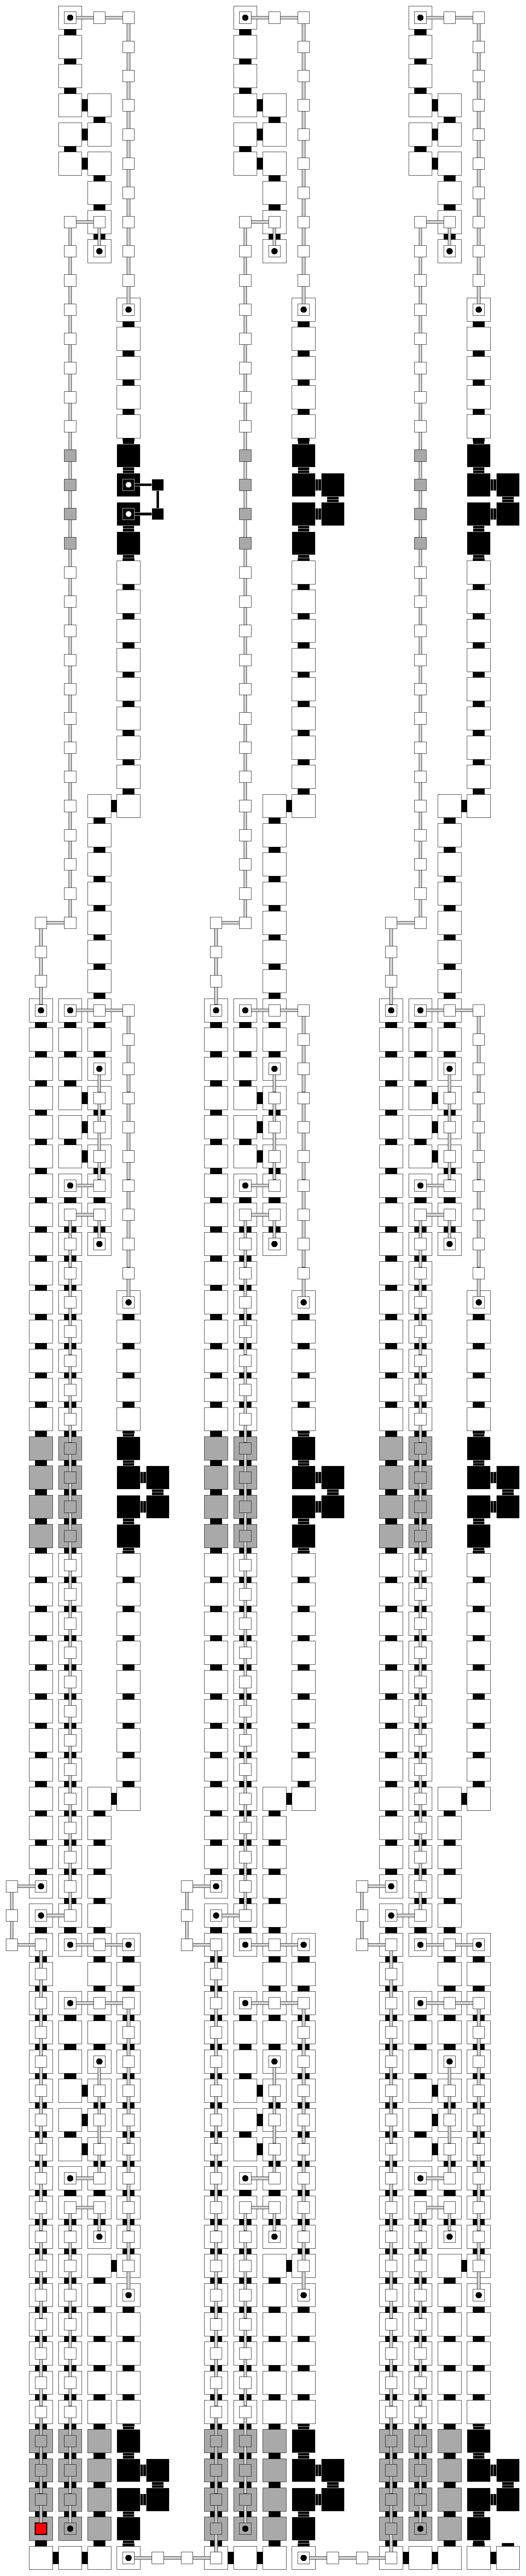
\includegraphics[width=0.3\textwidth]{seed/seed_overview_case3}
        \caption{\label{fig:initial_value_case3} Initial value case 3}
    \end{subfigure}%
    ~
    \begin{subfigure}[t]{0.3\textwidth}
        \centering
        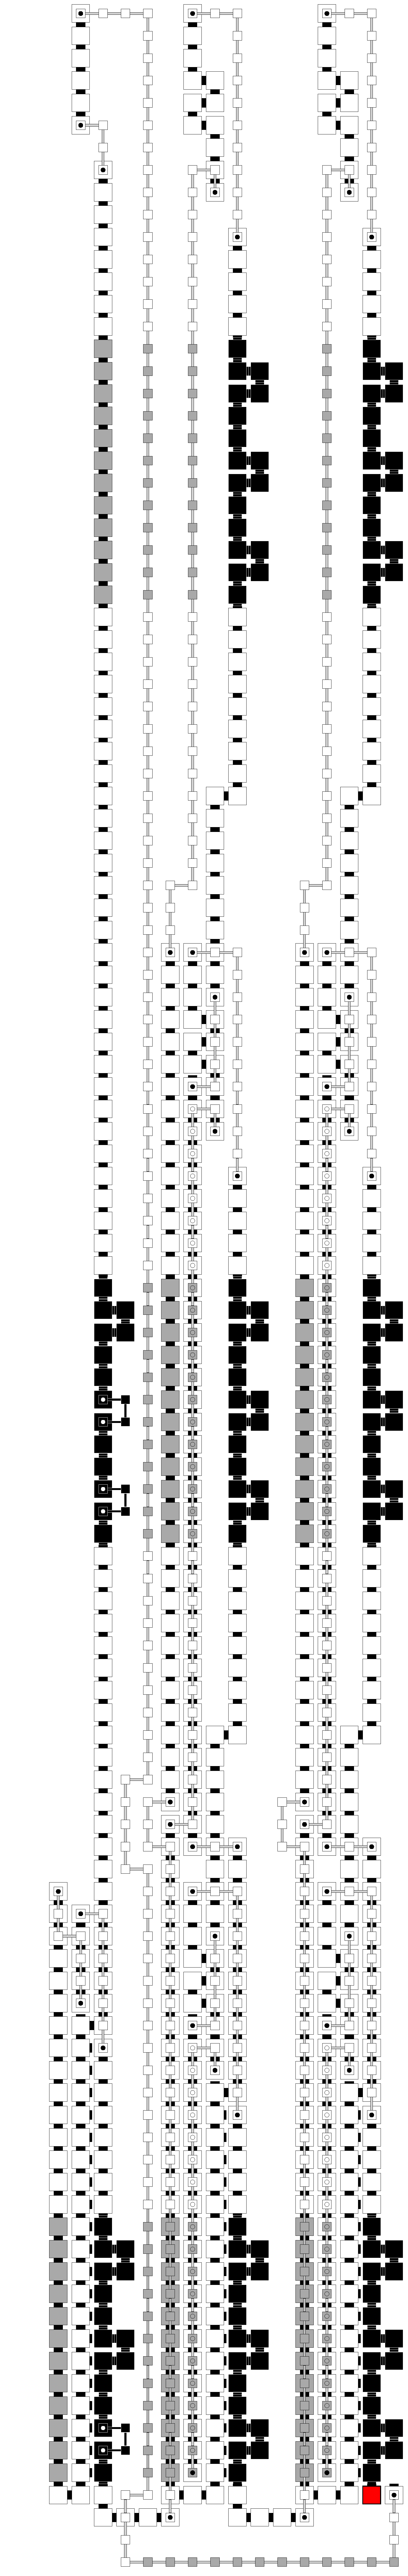
\includegraphics[width=0.3\textwidth]{seed/seed_overview_case2}
        \caption{\label{fig:initial_value_case2} Initial value case 2}
    \end{subfigure}%
    ~
    \begin{subfigure}[t]{0.3\textwidth}
        \centering
        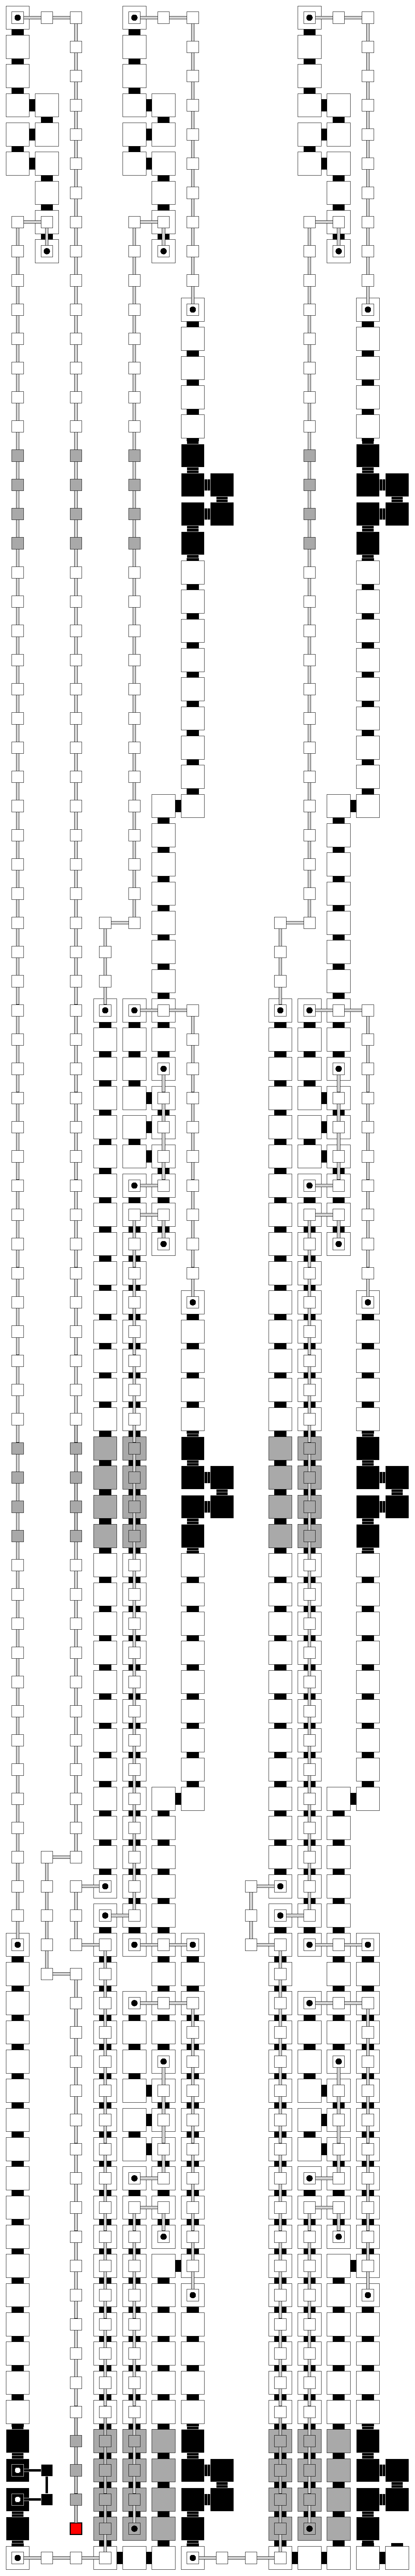
\includegraphics[width=0.3\textwidth]{seed/seed_overview_case1}
        \caption{\label{fig:initial_value_case1} Initial value case 1}
    \end{subfigure}%
    ~
\end{figure}
